\documentclass{standalone}
\usepackage{graphicx}	
\usepackage{amssymb, amsmath}
\usepackage{color}

\usepackage{tikz}
\usetikzlibrary{intersections, backgrounds, math}
\usepackage{pgfmath}

\definecolor{light}{RGB}{220, 188, 188}
\definecolor{mid}{RGB}{185, 124, 124}
\definecolor{dark}{RGB}{143, 39, 39}
\definecolor{darker}{RGB}{124, 0, 0}
\definecolor{highlight}{RGB}{180, 31, 180}
\definecolor{lightteal}{RGB}{186, 219, 219}
\definecolor{midteal}{RGB}{124, 186, 186}
\definecolor{darkteal}{RGB}{38, 142, 142}
\definecolor{darkerteal}{RGB}{0, 124, 124}
\definecolor{gray10}{gray}{0.1}
\definecolor{gray20}{gray}{0.2}
\definecolor{gray30}{gray}{0.3}
\definecolor{gray40}{gray}{0.4}
\definecolor{gray60}{gray}{0.6}
\definecolor{gray70}{gray}{0.7}
\definecolor{gray80}{gray}{0.8}
\definecolor{gray90}{gray}{0.9}
\definecolor{gray95}{gray}{0.95}

\begin{document}

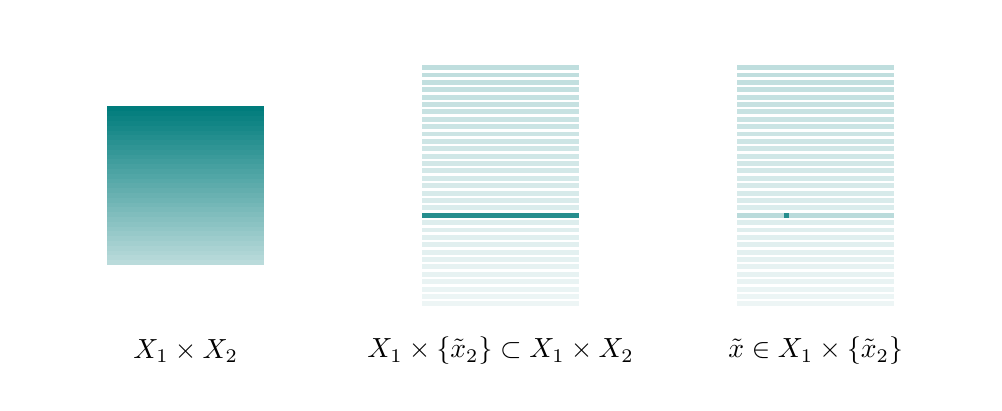
\begin{tikzpicture}[scale=1.0]
 
  \pgfmathsetmacro{\delta}{1 / 32}
  
  \begin{scope}[shift={(0, 0)}]
  
    \draw[white] (-2, -2.5) rectangle (2, 2);
    
    \foreach \n in {0, 1, ..., 32} {
      \pgfmathsetmacro{\eta}{0.975 * (\n / 16 - 1) + 0}
      \pgfmathsetmacro{\prop}{100 * \n / 32}
      \colorlet{custom}{darkerteal!\prop!lightteal}; 
      \fill[custom]    (-1, \eta - \delta) -- (-1, \eta + \delta) 
                    -- (+1, \eta + \delta) -- (+1, \eta - \delta);
    }
        
    \node at (0, -2.1) 
      { $X_{1} \times X_{2}$ };
    
  \end{scope}
  
  \begin{scope}[shift={(4, 0)}]
  
    \draw[white] (-2, -2.5) rectangle (2, 2);
    
    \foreach \n in {0, 1, ..., 32} {
      \pgfmathsetmacro{\eta}{1.5 * (\n / 16 - 1) + 0}
      \pgfmathsetmacro{\prop}{100 * \n / 32}
      \colorlet{custom}{darkerteal!\prop!lightteal}; 
      \fill[custom]    (-1, \eta - \delta) -- (-1, \eta + \delta) 
                    -- (+1, \eta + \delta) -- (+1, \eta - \delta);
    }
    
    \fill[white, opacity=0.75] (-2, -2.5) rectangle (2, 2);
    
    \foreach \n in {12} {
      \pgfmathsetmacro{\eta}{1.5 * (\n / 16 - 1) + 0}
      \fill[darkteal]    (-1, \eta - \delta) -- (-1, \eta + \delta) 
                      -- (+1, \eta + \delta) -- (+1, \eta - \delta);
    }
        
    \node at (0, -2.1) 
      { $X_{1} \times \{ \tilde{x}_{2} \} \subset X_{1} \times X_{2} $ };
    
  \end{scope}
  
  \begin{scope}[shift={(8, 0)}]
  
    \draw[white] (-2, -2.5) rectangle (2, 2);
    
    \foreach \n in {0, 1, ..., 32} {
      \pgfmathsetmacro{\eta}{1.5 * (\n / 16 - 1) + 0}
      \pgfmathsetmacro{\prop}{100 * \n / 32}
      \colorlet{custom}{darkerteal!\prop!lightteal}; 
      \fill[custom]    (-1, \eta - \delta) -- (-1, \eta + \delta) 
                    -- (+1, \eta + \delta) -- (+1, \eta - \delta);
    }
    
    \fill[white, opacity=0.75] (-2, -2.5) rectangle (2, 2);
    
    \foreach \n in {12} {
      \pgfmathsetmacro{\eta}{1.5 * (\n / 16 - 1) + 0}
      \fill[lightteal]    (-1, \eta - \delta) -- (-1, \eta + \delta) 
                       -- (+1, \eta + \delta) -- (+1, \eta - \delta);
      \fill[darkteal] (\eta - \delta, \eta - \delta) rectangle (\eta + \delta, \eta + \delta);
    }
        
    \node at (0, -2.1) 
      { $\tilde{x} \in X_{1} \times \{ \tilde{x}_{2} \}$ };
    
  \end{scope}


\end{tikzpicture}

\end{document}  